\documentclass[sigconf]{acmart}

% Remove/adjust for your submission venue as needed.
% \settopmatter{printacmref=false} % Removes ACM Reference Format
% \renewcommand\footnotetextcopyrightpermission[1]{} % removes copyright text

\usepackage{lmodern}
\usepackage{tikz}
\usetikzlibrary{arrows.meta, positioning}
\usepackage{tabularx}
\usepackage{booktabs}
\usepackage{url}

%\title{Towards Secure, Multitenant, Vendor-Neutral Enterprise RAG on Shared Infrastructure}
\title{Securing the Agent: Vendor-Neutral, Multitenant Enterprise Retrieval and Tool Use}

\author{Varsha Prasad}
\affiliation{%
  \institution{Red Hat AI}
  \city{Boston}
  \country{USA}
}
\email{vnarsing@redhat.com}

\author{Francisco Javier Arceo}
\affiliation{%
  \institution{Red Hat AI}
  \city{Boston}
  \country{USA}
}
\email{farceo@redhat.com}

\begin{abstract}
Retrieval-Augmented Generation (RAG) and agentic AI systems are increasingly prevalent in enterprise AI deployments. However, real enterprise environments introduce challenges largely absent from academic treatments and consumer-facing APIs: multiple tenants with heterogeneous data, strict access-control requirements, regulatory compliance, and cost pressures that demand shared infrastructure.

A fundamental problem underlies existing RAG architectures in these settings: dense retrieval ranks documents by semantic similarity, not by authorization---so a query from one tenant can surface another tenant's confidential data simply because it is the nearest neighbor. We formalize this gap and analyze additional failure modes---including tool-mediated disclosure, context accumulation across turns, and client-side orchestration bypass---that arise when agentic systems conflate relevance with authorization. To address these challenges, we introduce a layered isolation architecture combining policy-aware ingestion, retrieval-time gating, and shared inference, enforced through server-side agentic orchestration. Unlike client-side agent patterns, this approach centralizes tool execution, state management, and policy enforcement on the server, creating natural enforcement points for multitenant isolation and eliminating per-tenant infrastructure duplication.

An open-source implementation using Llama Stack---a vendor-neutral framework realizing the Responses API paradigm with server-side multi-turn orchestration---and its Kubernetes Operator demonstrates that secure multitenancy, cost-efficient sharing, and the flexibility of modern agentic systems are simultaneously achievable on shared infrastructure.
\end{abstract}

% TODO: update ACM classification.
\begin{CCSXML}
<ccs2012>
 <concept>
  <concept_id>10010147.10010257</concept_id>
  <concept_desc>Computing methodologies~Machine learning</concept_desc>
  <concept_significance>300</concept_significance>
 </concept>
 <concept>
  <concept_id>10002951.10003227.10003351</concept_id>
  <concept_desc>Information systems~Data management systems</concept_desc>
  <concept_significance>100</concept_significance>
 </concept>
</ccs2012>
\end{CCSXML}
\ccsdesc[300]{Computing methodologies~Machine learning}
\ccsdesc[100]{Information systems~Data management systems}

\keywords{Llama Stack, Kubernetes operator, LLM systems, MLOps, LLMOps}

\begin{document}
\maketitle

\section{Introduction}
\subsection{Motivation}
Enterprise adoption of generative AI has evolved beyond simple prompt-response interactions toward agentic systems---AI applications that autonomously reason, use tools, retrieve information, and execute multi-step workflows to accomplish complex tasks~\cite{yao2023react,schick2023toolformer,karpas2022mrkl}.
This evolution reflects a fundamental shift: rather than treating large language models (LLMs) as sophisticated text generators, organizations now deploy them as reasoning engines capable of taking actions in the world.

An API-first paradigm for these systems is to unify multi-turn inference, tool use, and retrieval behind a single endpoint.
OpenAI's Responses API has emerged as a de facto interface pattern for building such systems by providing a unified interface for chat-style inference, tool invocation, retrieval tools, and stateful workflows~\cite{openaiResponsesAPI}.
In parallel, open implementations increasingly expose OpenAI-compatible endpoints to decouple applications from a specific model provider.

However, real-world enterprise deployments differ sharply from the assumptions embedded in consumer-facing APIs and many academic prototypes.
Enterprise environments exhibit characteristics that demand specialized architectural consideration:
\begin{itemize}
  \item \textbf{Multiple tenants:} distinct business units, customers, or partners served from shared infrastructure, with strict isolation requirements.
  \item \textbf{Heterogeneous data:} document collections vary in format, sensitivity classification, and access requirements.
  \item \textbf{Strict access control:} regulatory frameworks require fine-grained governance with auditable access patterns.
  \item \textbf{Operational control:} visibility into agent behavior, tool execution sequences, and data access patterns is required for debugging and compliance, consistent with lessons from production ML engineering~\cite{amershi2019se4ml}.
  \item \textbf{Vendor independence:} lock-in to a single AI provider creates business risk; enterprises require on-prem and hybrid options.
\end{itemize}

Na\"{\i}ve approaches to addressing these requirements replicate the entire agentic stack per tenant: separate vector stores, dedicated inference endpoints, and isolated tool configurations.
This strategy incurs substantial costs --- infrastructure scales linearly with tenants rather than with actual usage --- and creates operational fragmentation that amplifies common ML systems maintenance risks~\cite{sculley2015hiddentechnicaldebt}.

\subsection{Problem statement}
This paper addresses a fundamental tension in enterprise agentic AI deployment:

\begin{quote}
Enterprises require both shared infrastructure for cost efficiency and strict tenant isolation for security and compliance --- while maintaining the flexibility of modern agentic architectures.
\end{quote}

Standard agentic AI deployments exhibit assumptions incompatible with this requirement:
\begin{enumerate}
  \item \textbf{Client-side orchestration:} the application manages the inference--tool--inference loop, distributing security-critical logic to potentially untrusted clients and increasing operational complexity~\cite{amershi2019se4ml}.
  \item \textbf{Homogeneous data access:} retrieval stacks assume uniform access to a corpus; dense retrieval methods (e.g., DPR) optimize similarity ranking rather than authorization~\cite{karpukhin2020dpr}.
  \item \textbf{Implicit trust boundaries:} tool execution is often treated as a capability extension without systematic verification of who may invoke tools or consume tool outputs, despite the centrality of tool use in modern agent designs~\cite{yao2023react,schick2023toolformer,karpas2022mrkl}.
  \item \textbf{Stateless isolation:} requests are treated independently, ignoring how conversation state and cached tool results can leak across boundaries; such hidden couplings are a classic source of ML systems fragility~\cite{sculley2015hiddentechnicaldebt}.
\end{enumerate}

In multitenant settings, these assumptions create serious vulnerabilities.
A document highly similar to a query may belong to a different tenant.
A tool call may access resources outside the user's authorization scope.
Conversation history may accumulate context that crosses security boundaries.

\subsection{Contributions}
This paper makes the following contributions:
\begin{enumerate}
  \item We formalize the problem of \emph{multitenant enterprise RAG} under shared infrastructure, showing why semantic similarity alone (as used by dense retrievers and ANN indexes) is insufficient to enforce isolation and authorization~\cite{karpukhin2020dpr,johnson2017faiss}.

  \item We analyze failure modes of existing RAG and agentic systems in multitenant settings, including cross-tenant retrieval leakage, unauthorized context construction, and policy violations arising from client-side orchestration.

  \item We propose a layered isolation architecture for enterprise RAG that combines policy-aware ingestion, retrieval-time gating, and shared inference to achieve strict tenant isolation without per-tenant duplication of storage or models.

  \item We introduce server-side orchestration as a unifying enforcement layer that centralizes retrieval, tool execution, and state management, reducing the trusted computing base for secure multitenant RAG and aligning with production ML engineering best practices~\cite{sculley2015hiddentechnicaldebt,amershi2019se4ml}.

  \item We present an open-source, vendor-neutral framework based on Llama Stack~\cite{llamastack} and Kubernetes deployment via an operator~\cite{llamastackk8soperator,burns2016borg} that enables pluggable models, vector stores, and tools, demonstrating the feasibility of secure multitenant RAG on shared infrastructure.
\end{enumerate}

\paragraph{Primary sources.}
Llama Stack~\cite{llamastack}: \url{https://github.com/llamastack/}.\\
Kubernetes operator~\cite{llamastackk8soperator}: \url{https://github.com/llamastack/llama-stack-k8s-operator}.

\section{Background and Related Work}
\subsection{The evolution of LLM application architectures}
LLM application architectures have evolved through distinct phases, each introducing new capabilities and security considerations.
\textbf{Completion APIs} exposed simple prompt\,$\rightarrow$\,text interfaces with perimeter-oriented security.

\textbf{Retrieval-augmented generation (RAG)}~\cite{lewis2020rag} introduced retrieval and new attack surfaces such as retrieval manipulation and context poisoning.
\textbf{Dense retrieval and learned retrievers} (e.g., DPR~\cite{karpukhin2020dpr} and retrieval-augmented pretraining such as REALM~\cite{guu2020realm}) established the core technical basis for modern RAG.
\textbf{Vector search infrastructure} (e.g., FAISS~\cite{johnson2017faiss}) enabled ANN retrieval at scale.
\textbf{Tool-using agents}~\cite{yao2023react,schick2023toolformer,karpas2022mrkl} extended LLMs with tool calls and an inference\,$\rightarrow$\,tool\,$\rightarrow$\,inference loop.
\textbf{Autonomous multi-step agents} execute multi-tool workflows with limited human oversight.
In multitenant deployments, isolation must span retrieval, tool invocation, state accumulation, and orchestration.

\subsection{The Responses API paradigm}
The Responses API establishes conventions for agentic applications:
(1) a unified tool interface with typed schemas,
(2) integrated retrieval as a first-class tool,
(3) stateful conversations for multi-session workflows, and
(4) streaming events for visibility~\cite{openaiResponsesAPI}.
The paradigm unifies chat, retrieval, and tool use, but common reference deployments assume a single-tenant trusted client and do not address policy-aware retrieval gating or tenant-scoped state isolation.

\subsection{Multitenancy in AI infrastructure}
Multitenancy is well-studied in databases (e.g., row-level security), cloud platforms (namespaces, RBAC), and ML serving (quotas and routing), but agentic AI adds new requirements.
Isolation must span not just data retrieval but tool execution, state management, and orchestration logic.
Kubernetes has become the de facto substrate for shared infrastructure, building on lessons from cluster managers such as Borg and Omega~\cite{burns2016borg}.
At the serving layer, LLM inference efficiency and scheduling can dominate both latency and cost, motivating modern serving systems and memory-management approaches~\cite{kwon2023vllm,yu2022orca}.

\subsection{Access control in AI systems}
Traditional access control focuses on API boundaries (authentication, authorization, rate limiting).
In agentic systems, internal decisions (retrieval, tool invocation, evidence admission) must also be policy-aware.
Production ML practice shows that unclear boundaries and implicit couplings are recurrent sources of operational risk~\cite{sculley2015hiddentechnicaldebt,amershi2019se4ml}.
The problem of policy-aware agentic execution in multitenant settings remains underexplored.

\section{Problem Definition: Multitenant Enterprise Agentic AI}
\subsection{System model}
We formalize the multitenant agentic AI environment.
Tenants ($T$) share infrastructure; each tenant $t \in T$ has associated data, users, tools, and policies.
Users ($U$) submit requests and possess attributes $A_u$ (roles, clearances, group memberships).
Documents ($D$) live in vector stores with metadata (tenant ownership, classification, access policy).
Tools ($\Phi$) include retrieval (\texttt{file\_search}), web access (\texttt{web\_search}), remote services (MCP), and custom functions.
Policies ($P$) govern access (document access, tool invocation, and fine-grained actions).
Agent execution is a sequence of inference and tool steps as in tool-using agent formulations~\cite{yao2023react,karpas2022mrkl}:
\[
E = [(i_1, \phi_1, r_1), (i_2, \phi_2, r_2), \dots, (i_n, \emptyset, r_n)].
\]

\subsection{Threat model and key risks}
We consider cross-tenant data leakage via retrieval, tool-mediated disclosure, context accumulation attacks, client-side orchestration bypass, state leakage across sessions, relevance distortion, and audit failure.

\subsection{Limitations of client-side orchestration}
In the standard client-managed loop, the client executes tools and returns tool results, which distributes trust to every client.
A malicious client can fabricate tool results, inject unauthorized context, skip security-critical tools, or manipulate conversation state.
For enterprise multitenancy, client-side orchestration is fundamentally unsuitable.

\subsection{The case for server-side orchestration}
Server-side orchestration centralizes tool execution, state management, and policy enforcement within the trust boundary and enables a complete audit trail.
This model matches the control-plane needs implied by multi-step tool-using agents~\cite{yao2023react,schick2023toolformer,karpas2022mrkl} while reducing the operational surface area highlighted in production ML systems research~\cite{amershi2019se4ml}.

\section{Limitations of Common Solutions in Multitenant Enterprise Settings}
\label{sec:common-limitations}

This section discusses limitations of common frameworks and deployment patterns---LangChain, LlamaIndex, OpenAI API, and naive RAG stacks---when applied to multitenant enterprise settings. The goal is to explain why typical, out-of-the-box patterns are not sufficient for enterprise multitenancy, motivating the architecture proposed in Section~\ref{sec:layered-arch}. Each limitation is illustrated with a concrete scenario drawn from how existing tools work today; residual limitations of our approach are discussed in Section~9.

Every major RAG framework retrieves documents by semantic similarity (cosine distance or dot product) using dense retrievers such as DPR~\cite{karpukhin2020dpr} and ANN indexing techniques commonly implemented in vector search libraries (e.g., FAISS)~\cite{johnson2017faiss}.
Similarity is orthogonal to authorization: a document from tenant $B$ may be the most semantically similar result for tenant $A$'s query, yet returning it violates isolation. This is a structural property of similarity ranking, independent of the specific framework.

Formally, let tenants $T_A$ and $T_B$ share a corpus $D = D_A \cup D_B$, and let $q$ be a query from user $u_A \in T_A$. Denote by $\mathrm{sim}(q,d)$ the similarity score and by $\mathrm{tenant}(d)$ the tenant owning document $d$. The isolation invariant requires that only documents with $\mathrm{tenant}(d) = \mathrm{tenant}(u_A)$ be returned. For any similarity threshold $\theta$ and any $k \geq 1$, there exist queries $q$ such that $\arg\max_{d \in D} \mathrm{sim}(q,d) \in D_B$; that is, the top result belongs to the wrong tenant. Thus similarity-based retrieval without an authorization predicate cannot enforce tenant isolation. Retrieval must be composed with a policy check: $\mathcal{R}(q,u) = \{ d \in D : \mathrm{sim}(q,d) > \theta \wedge P(u,d) = \mathrm{permit} \}$.

\begin{figure}[t]
  \centering
  \resizebox{\columnwidth}{!}{%
  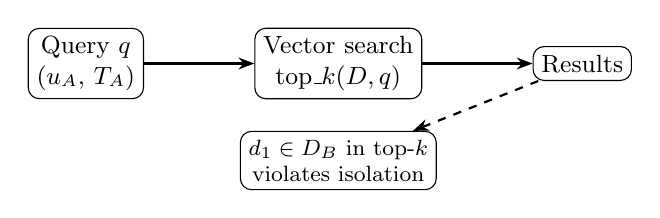
\begin{tikzpicture}[
    box/.style={draw, rounded corners, align=center, inner sep=3pt, font=\small},
    arrow/.style={-{Stealth[length=2.0mm]}, thick}
  ]
    \node[box] (query) {Query $q$\\($u_A$, $T_A$)};
    \node[box, right=14mm of query] (vs) {Vector search\\$\mathrm{top}\_k(D, q)$};
    \node[box, right=14mm of vs] (out) {Results};
    \node[box, below=4mm of vs, font=\footnotesize] (leak) {$d_1 \in D_B$ in top-$k$\\violates isolation};
    \draw[arrow] (query) -- (vs);
    \draw[arrow] (vs) -- (out);
    \draw[arrow, dashed] (out) -- (leak);
  \end{tikzpicture}%
  }
  \caption{Similarity-only retrieval: top-$k$ from shared corpus $D$ can include documents from another tenant ($d_1 \in D_B$), violating isolation.}
  \label{fig:similarity-leak}
\end{figure}

\subsection{Cross-tenant retrieval risk}
Any RAG framework that uses a shared vector store across tenants without mandatory metadata filtering exhibits this failure.
Tenant $A$'s query can retrieve tenant $B$'s confidential documents because they are semantically similar under dense retrieval~\cite{karpukhin2020dpr} and selected via ANN ranking~\cite{johnson2017faiss}.
Even when systems support metadata filters, filtering is often optional and client-controlled; a developer can omit the filter.
The root cause is that vector search ranks by embedding distance, not ownership; filtering is an opt-in afterthought rather than an architectural invariant.

\subsection{Unauthorized context construction}
Multi-turn agent frameworks persist conversation history without re-validating access policies per turn.
Documents retrieved in turn 1 remain in the conversation context when turn 2 executes.
If permissions change between turns (e.g., access revoked, user role changed), stale context from turn 1 is still available to the LLM.
This resembles broader production ML issues where data and state dependencies are implicit and difficult to govern over time~\cite{sculley2015hiddentechnicaldebt,amershi2019se4ml}.

\subsection{Tool-mediated disclosure risk}
Agent frameworks with tool or function calling execute tools with the agent's credentials, not the end user's.
An agent may invoke a tool (e.g., database query, API call, MCP server) that returns data the requesting user is not authorized to see; the tool result is included in the LLM context and may appear in the response.
This risk is amplified by agent designs that interleave reasoning with actions and tool outputs~\cite{yao2023react,karpas2022mrkl} and by approaches that encourage models to autonomously decide when to invoke tools~\cite{schick2023toolformer}.
There is no standard mechanism for per-invocation user-level authorization in many deployed stacks.

\subsection{Client-side orchestration trust gap}
When the inference--tool--inference loop runs in the client (or tenant-controlled backend), a malicious or buggy client can skip retrieval filters, invoke tools directly, or modify the agent loop to extract unauthorized data.
The trusted computing base (TCB) in client-side orchestration includes the client code, which is outside the security boundary.
This design also exacerbates the operational complexity documented in production ML engineering case studies~\cite{amershi2019se4ml}.

\subsection{State isolation risk across sessions}
Frameworks with persistent memory or state deployed on shared infrastructure can leak conversation state, cached tool results, or response history from one tenant's session to another when storage lacks proper isolation.
Existing frameworks often delegate persistence to the developer, who must manually implement isolation; a single missed filter can leak entire conversation histories.
This is consistent with well-known failure modes where data and configuration coupling introduce hidden dependencies and maintenance hazards~\cite{sculley2015hiddentechnicaldebt}.

\subsection{Audit and compliance gaps}
In regulated enterprise environments, an enterprise must demonstrate which documents were retrieved, which tools were invoked, and which policies were evaluated for a given response.
With client-side orchestration, execution is distributed across the client app, vector store, LLM API, and tool endpoints with no single point of observability.
This problem aligns with the broader call for systematic software engineering practices for ML systems, including monitoring and end-to-end traceability~\cite{amershi2019se4ml}.

\section{Layered Isolation Architecture}
\label{sec:layered-arch}

We propose a three-layer architecture that directly addresses the failure modes identified in Section~\ref{sec:common-limitations}: policy-aware ingestion, retrieval-time gating, and shared inference.

\subsection{Policy-aware ingestion (Layer 1)}
Tenant metadata must be attached at document ingestion time, not retrofitted.
This reduces the risk of accidental cross-tenant coupling and missing invariants during system evolution~\cite{sculley2015hiddentechnicaldebt}.
Define an ingestion function $\mathcal{I}(d, t) \rightarrow D_t$ that tags document $d$ with tenant $t$'s attributes so that every chunk inherits ownership metadata.
In Llama Stack, when files are attached to vector stores, the \texttt{attributes} parameter carries tenant ownership, classification, and access policy; these are stored as chunk metadata.

\subsection{Retrieval gating (Layer 2)}
Retrieval is gated in two tiers.
\textbf{(1) Resource-level ABAC:} before any search, the system checks that the user is authorized to read the vector store; if not, no search is performed.
\textbf{(2) Chunk-level metadata filtering:} after retrieval, structured filters are applied on chunk metadata so that only documents satisfying the policy are admitted.
This composes similarity search (dense retrieval~\cite{karpukhin2020dpr} over ANN indexes~\cite{johnson2017faiss}) with a mandatory authorization predicate:
\[
\mathcal{R}(q,u) = \{ d \in D : \mathrm{sim}(q,d) > \theta \wedge P(u,d) = \mathrm{permit} \}.
\]
Backends such as Elasticsearch and SQL-backed vector stores can support predicate pushdown for efficiency on large corpora; otherwise, post-retrieval gating still enforces the semantic/authorization separation.

\subsection{Shared inference (Layer 3)}
The LLM inference layer is shared across tenants; the model itself does not require per-tenant isolation, only the context fed to it.
Because layers 1 and 2 ensure that only authorized documents and tool results enter the prompt, the inference layer can be safely shared.
At the serving layer, modern systems show that batching, scheduling, and memory management dominate throughput and latency for generative transformers~\cite{yu2022orca,kwon2023vllm}.
With $N$ tenants and $M$ model endpoints, cost scales as $O(M)$ rather than $O(N \cdot M)$.

\section{Server-Side Orchestration as Enforcement Layer}
\label{sec:server-side}

Server-side orchestration is essential for multitenant security: it centralizes retrieval, tool execution, and state management, reducing the trusted computing base and addressing failure modes in Section~\ref{sec:common-limitations}.
This design also aligns with the execution structure implied by tool-using agent formulations~\cite{yao2023react,karpas2022mrkl}.

\subsection{The case against client-side orchestration}
In client-side patterns, the client controls the inference--tool--inference loop.
A compromised or buggy client can skip retrieval filters, invoke unauthorized tools, or accumulate cross-tenant context.
Formally, client-side orchestration expands the TCB to include untrusted client code, so server-side security invariants cannot be enforced from the server alone.
This is consistent with broader findings that ML systems become fragile when critical invariants are distributed across components without clear ownership or enforcement points~\cite{sculley2015hiddentechnicaldebt,amershi2019se4ml}.

\subsection{Server-side orchestration in Llama Stack}
Llama Stack implements the Responses API with the full loop executed on the server~\cite{llamastack,openaiResponsesAPI}.
Tool execution (\texttt{file\_search}, \texttt{web\_search}, MCP, and function tools) runs inside the server trust boundary, and state is managed server-side with tenant-scoped access control.
Streaming events expose tool calls and text deltas, improving observability in line with production ML monitoring and governance needs~\cite{amershi2019se4ml}.

\begin{figure}[t]
    \centering
    \resizebox{\columnwidth}{!}{%
    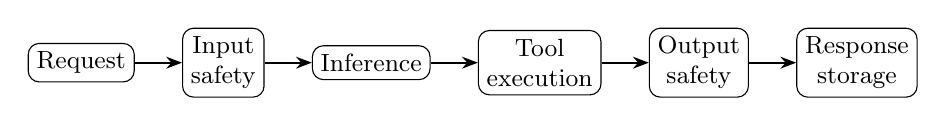
\begin{tikzpicture}[
      box/.style={draw, rounded corners, align=center, inner sep=3pt, font=\small},
      arrow/.style={-{Stealth[length=2.0mm]}, thick}
    ]
      \node[box] (req) {Request};
      \node[box, right=6mm of req] (in) {Input\\safety};
      \node[box, right=6mm of in] (inf) {Inference};
      \node[box, right=6mm of inf] (tool) {Tool\\execution};
      \node[box, right=6mm of tool] (out) {Output\\safety};
      \node[box, right=6mm of out] (store) {Response\\storage};
      \draw[arrow] (req) -- (in);
      \draw[arrow] (in) -- (inf);
      \draw[arrow] (inf) -- (tool);
      \draw[arrow] (tool) -- (out);
      \draw[arrow] (out) -- (store);
    \end{tikzpicture}%
    }
    \caption{Server-side orchestration flow: every step runs inside the server trust boundary.}
    \label{fig:orchestration-flow}
  \end{figure}

\subsection{Enforcement points}
Table~\ref{tab:enforcement} maps each failure mode from Section~\ref{sec:common-limitations} to the enforcement point that mitigates it.

\begin{table}[t]
  \centering
  \small
  \setlength{\tabcolsep}{3pt}
  \renewcommand{\arraystretch}{1.1}
  \begin{tabularx}{\columnwidth}{@{}l|X@{}}
  \toprule
  Failure mode & Enforcement point \\
  \midrule
  Cross-tenant retrieval leakage & Layer 2 retrieval gating (ABAC + metadata filters) composed with dense retrieval~\cite{karpukhin2020dpr} \\
  \midrule
  Unauthorized context construction & Tenant-scoped state storage and per-turn authorization (motivated by production ML pitfalls~\cite{sculley2015hiddentechnicaldebt,amershi2019se4ml}) \\
  \midrule
  Tool-mediated disclosure & Server-side tool execution with authorization propagation, aligned with tool-using agent loops~\cite{yao2023react,schick2023toolformer} \\
  \midrule
  Client-side bypass & Server-side orchestration (reduced TCB) \\
  \midrule
  State leakage & Per-user / per-tenant state isolation in the server-side store \\
  \midrule
  Audit failure & Server-side telemetry and tracing (production ML governance needs~\cite{amershi2019se4ml}) \\
  \bottomrule
  \end{tabularx}
  \caption{Mapping from failure modes to architectural enforcement points.}
  \label{tab:enforcement}
\end{table}

\subsection{Safety and guardrails integration}
Input and output guardrails run before inference (input) and after response generation (output). Shield providers can include inline and remote safety components; regardless of provider choice, server-side orchestration makes safety enforcement uniform and auditable.

\section{Reference Architecture: Llama Stack}
\label{sec:ref-arch}

This section presents Llama Stack~\cite{llamastack} as a reference architecture for secure, multitenant agentic AI systems. Llama Stack is an open-source, vendor-neutral framework that provides a unified API layer for building agentic applications while centralizing orchestration, policy enforcement, and access control. Unlike client-side orchestration libraries, Llama Stack executes the agentic control loop entirely on the server, creating natural enforcement points for multitenancy, security, and compliance. Kubernetes-native deployment follows established patterns for shared-cluster infrastructure~\cite{burns2016borg} and is automated via an operator~\cite{llamastackk8soperator}.

While the architectural principles described in this section are general, Llama Stack serves as a concrete instantiation that demonstrates their feasibility on shared Kubernetes infrastructure.

\subsection{Design Philosophy}
Llama Stack emerged from the observation that the LLM application ecosystem had become fragmented, with overlapping component implementations, incompatible interfaces, and limited end-to-end coverage of the model lifecycle. In response, the framework adopts four core design principles.

First, Llama Stack follows an API-first design. All capabilities are exposed through well-defined, versioned APIs that mirror widely adopted industry standards, such as OpenAI-compatible endpoints, while extending them to support enterprise requirements including multitenancy, policy enforcement, and observability.

Second, the framework adopts a pluggable provider model. Each API is implemented by interchangeable providers that share a common interface, enabling vendor independence and hybrid deployments across on-premise and cloud environments.

Third, Llama Stack implements server-side agentic orchestration. The full agentic execution loop—including inference, tool invocation, and subsequent inference—executes within the server trust boundary. This design contrasts with client-side orchestration approaches and enables centralized enforcement of access control, safety policies, and execution constraints.

Finally, the framework introduces a distribution model. Pre-configured combinations of APIs and providers are packaged as distributions, enabling turnkey deployment while preserving flexibility for customization and provider substitution.

\subsection{Layered Architecture}
Llama Stack follows a layered architecture that separates concerns across distinct tiers, as illustrated in Figure~\ref{fig:architecture}. At the top, an HTTP/REST layer handles request routing, authentication, quota enforcement, and streaming. Beneath this layer, a set of domain-specific APIs expose functionality for inference, agentic execution, vector I/O, safety, and tool integration.

A routing layer mediates between API calls and concrete provider implementations, resolving logical resource identifiers (e.g., model identifiers or vector store identifiers) to physical provider instances. Below this, a provider layer encapsulates both inline providers executing in-process and remote providers that adapt external services. Persistent state is maintained in a storage layer comprising key–value stores, relational stores, and vector databases.

This separation enables independent evolution of APIs, providers, and storage backends while preserving a unified control plane for policy enforcement.

\subsection{Core APIs and Agentic Execution}
Llama Stack defines a comprehensive set of APIs covering the full lifecycle of agentic applications, including inference, agents, vector I/O, safety, tools, file management, and evaluation. Each API is designed with multitenancy as a first-class concern, enabling tenant-scoped resource management and access control.

The Agents API, which implements the OpenAI Responses API paradigm, is particularly significant for multitenant agentic systems. Unlike traditional chat completion APIs that terminate after a single inference call, the Responses API orchestrates complete agentic workflows. A single request may trigger multiple inference calls, tool executions, safety checks, and state transitions before producing a final response.

All such operations are executed within the server boundary. Conversation state is retrieved and persisted server-side, tools are invoked under centralized authorization, and safety guardrails are applied at each step. This design ensures that intermediate context, tool outputs, and execution state remain subject to uniform access control policies.

\subsection{Provider Architecture}
Extensibility in Llama Stack is achieved through its provider architecture. Each API may be backed by multiple providers, which are categorized as inline or remote. Inline providers execute within the Llama Stack process and are suitable for sensitive operations requiring in-process execution. Remote providers adapt external inference engines, vector databases, or services through standardized interfaces.

This separation enables hybrid deployments in which sensitive data paths remain local while computationally intensive operations are delegated to scalable external services. Crucially, provider substitution is transparent to clients, as all interactions occur through the unified API layer.

\subsection{Routing Layer}
The routing layer dispatches API requests to provider instances based on logical resource identifiers. For example, inference requests are routed according to model identifiers, while vector queries are routed based on vector store identifiers. This indirection enables fine-grained control over resource access and placement.

From a multitenancy perspective, the routing layer serves as a critical enforcement point. Routing decisions can incorporate authorization checks, tenant identity, and policy constraints before delegating requests to providers. Different tenants may thus be routed to distinct provider instances or storage backends while sharing the same API surface.

\subsection{Distribution Model}
A distribution packages a specific set of APIs, provider configurations, and registered resources into a deployable unit. Distributions support turnkey deployment for common scenarios, environment-specific configuration (e.g., development versus production), and seamless provider substitution without application changes.

By decoupling application logic from provider selection, the distribution model enables organizations to evolve their infrastructure and vendor choices while preserving stable interfaces for agentic applications.

\subsection{Access Control Framework}
Llama Stack includes a declarative, policy-based access control framework that evaluates authorization decisions at runtime. Policies specify permitted and forbidden actions over resource scopes, with conditions based on user identity, resource attributes, and ownership relationships.

Authorization checks are enforced at multiple layers, including API routes, routing table resolution, and tool execution. A default-deny model ensures that access is only granted when explicitly permitted by policy. This design enables consistent enforcement across inference, retrieval, and agentic execution.

\subsection{Server Architecture}
The Llama Stack server is implemented atop a modern asynchronous web framework and provides OpenAI-compatible endpoints for inference and agentic execution. Authentication middleware supports pluggable identity providers, while quota management enables per-principal rate limiting and usage tracking. Streaming execution is supported for long-running agentic workflows, and telemetry integration enables end-to-end observability.

Importantly, all agentic orchestration occurs within the server process, enabling comprehensive audit logging of inference calls, tool executions, and data access events.

\subsection{Implications for Multitenant Agentic AI}
Taken together, these architectural choices yield several properties essential for multitenant enterprise deployments. First, centralized orchestration creates uniform enforcement points for access control and policy compliance. Second, provider-level isolation enables tenant-specific routing while preserving shared infrastructure. Third, server-managed state prevents cross-tenant context leakage across multi-turn interactions. Finally, centralized execution enables comprehensive auditing and compliance monitoring.

These properties form the foundation for the layered isolation architecture described in the following section, where we show how policy-aware ingestion, retrieval gating, and server-side orchestration can be composed to achieve secure, cost-efficient multitenant agentic AI.


\subsection{High-level architecture}
We propose a layered architecture for secure multitenant agentic AI with an authentication layer, a server-side agentic orchestrator, policy evaluation, and a shared-but-logically-isolated vector store.

\begin{figure}[t]
  \centering
  \resizebox{\columnwidth}{!}{%
  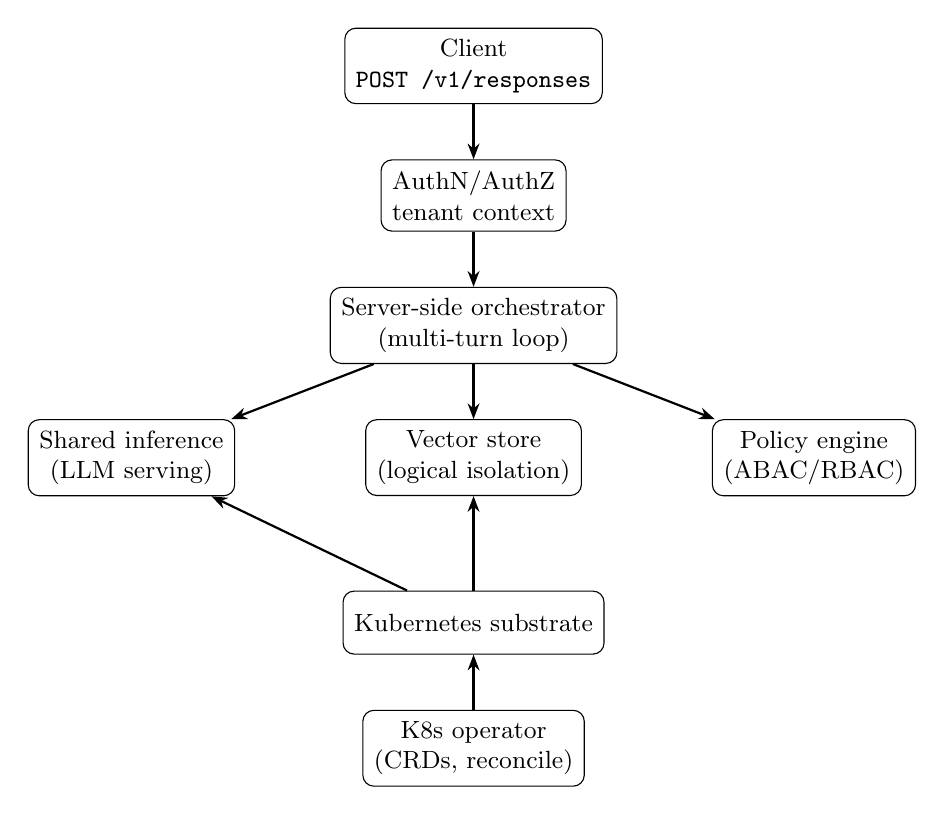
\begin{tikzpicture}[
    box/.style={draw, rounded corners, align=center, inner sep=4pt, minimum height=8mm, font=\small},
    arrow/.style={-{Stealth[length=2.0mm]}, thick}
  ]
    \node[box] (client) {Client\\\texttt{POST /v1/responses}};
    \node[box, below=7mm of client] (auth) {AuthN/AuthZ\\tenant context};
    \node[box, below=7mm of auth] (orch) {Server-side orchestrator\\(multi-turn loop)};

    \node[box, below left=7mm and 12mm of orch] (infer) {Shared inference\\(LLM serving)};
    \node[box, below=7mm of orch] (vec) {Vector store\\(logical isolation)};
    \node[box, below right=7mm and 12mm of orch] (policy) {Policy engine\\(ABAC/RBAC)};

    \node[box, below=12mm of vec] (k8s) {Kubernetes substrate};
    \node[box, below=7mm of k8s] (op) {K8s operator\\(CRDs, reconcile)};

    \draw[arrow] (client) -- (auth);
    \draw[arrow] (auth) -- (orch);

    \draw[arrow] (orch) -- (infer);
    \draw[arrow] (orch) -- (vec);
    \draw[arrow] (orch) -- (policy);

    \draw[arrow] (op) -- (k8s);
    \draw[arrow] (k8s) -- (infer);
    \draw[arrow] (k8s) -- (vec);
  \end{tikzpicture}%
  }
  \caption{Reference architecture for multitenant enterprise agentic AI on shared Kubernetes infrastructure.}
  \label{fig:architecture}
\end{figure}


\subsection{Authentication and tenant context}
Requests begin with authentication establishing a user and tenant context.
Claims (tenant/namespace, roles/groups, projects) are mapped to authorization attributes and propagated through the request lifecycle.

\subsection{Server-side agentic orchestration}
The orchestrator executes the multi-turn loop server-side: inference, tool-call detection, tool classification, policy evaluation, tool execution, and context construction.
Server-side tools (e.g., \texttt{file\_search}, \texttt{web\_search}, MCP tools) are executed within the trust boundary; client-side function tools are explicitly delegated.

\subsection{Policy-aware ingestion}
Ingestion attaches mandatory metadata (tenant attribution, classification) and records lineage for audit.
Documents without required metadata are rejected.

\subsection{Shared vector store with logical isolation}
A single physical vector index is shared, but each chunk carries tenant and policy metadata.
Retrieval uses query-time predicates (tenant predicates and classification filters) to prevent cross-tenant candidate leakage, separating similarity ranking from authorization checks~\cite{karpukhin2020dpr,johnson2017faiss}.

\subsection{Two-phase retrieval: search and admission}
Phase~1 performs filtered similarity search, grounded in dense retrieval and ANN indexing methods~\cite{karpukhin2020dpr,johnson2017faiss}.
Phase~2 applies policy-based admission; only admitted documents enter the generation context, and denials are logged.

\subsection{Tool execution with policy gating}
Every tool invocation is preceded by policy evaluation over user attributes, tool identity, and parameters.
This is particularly important for agent loops where the model chooses actions and tools iteratively~\cite{yao2023react,schick2023toolformer,karpas2022mrkl}.

\subsection{Shared inference with isolated contexts}
LLM instances are shared across tenants, but each request constructs an isolated context containing only authorized inputs.
Serving efficiency and scheduling are handled by the inference backend; modern LLM serving systems show that batching and memory management dominate throughput~\cite{yu2022orca,kwon2023vllm}.
Because isolation is enforced at ingestion and retrieval, the inference layer itself does not need per-tenant replicas—reducing cost to $O(M)$ model endpoints for $N$ tenants while preserving strict logical isolation.

\subsection{Overview and implementation}
Llama Stack is an open-source framework implementing the Responses API paradigm with server-side orchestration~\cite{llamastack,openaiResponsesAPI}.
It is vendor-neutral via a provider abstraction, and is designed for Kubernetes-native deployment and operator-based lifecycle management~\cite{llamastackk8soperator,burns2016borg}.

\subsection{Responses API implementation}
The Responses API exposes operations to create responses (execute an agent), retrieve responses, list responses, inspect input items, and delete responses; creation supports both streaming and non-streaming modes.
Internally, the implementation converts request input to chat messages and runs the inference--tool loop via a streaming orchestrator or a synchronous path.
Results are persisted through a responses store backed by an authorized SQL layer so that rows are tagged with owner and access attributes and filtered on read by the default ABAC policy.
Streaming events expose reasoning, tool calls, and text deltas, giving operators and auditors fine-grained visibility into agent behavior without requiring client-side instrumentation.

\subsection{Vector store abstraction and filters}
Llama Stack defines a vector store protocol (vector I/O API) implemented by multiple providers (e.g., Chroma, pgvector, Elasticsearch, in-process SQLite).
Each vector store is a logical resource registered in a routing table and subject to the same access control as other resources; creation assigns an owner from the authenticated user.
The protocol supports a structured filter language for query-time metadata constraints: comparison operators (\texttt{eq}, \texttt{ne}, \texttt{gt}, \texttt{gte}, \texttt{lt}, \texttt{lte}) and compound \texttt{and}/\texttt{or} filters.
When the agent uses \texttt{file\_search}, the server applies the user's tenant and policy attributes so that retrieval is gated by both resource-level and chunk-level checks, enabling metadata-driven isolation without requiring a separate physical index per tenant.

\subsection{Attribute-based access control}
Llama Stack supports ABAC-style policies for tenant isolation, role-based capabilities, and classification enforcement.
The access control engine evaluates \texttt{Access\-Rule}s with permit/forbid scopes and optional conditions (e.g., ``user in owners roles'', ``user is owner'', ``resource is unowned''); the default policy permits access when the user is the resource owner or when the user's attributes (roles, teams, projects, namespaces) match the resource's access attributes.
Authorization is enforced at API routes (e.g., \texttt{Route\-Authorization\-Middleware}), at routing table resolution (e.g., before resolving a vector store or model), and at storage read time via \texttt{Authorized\-Sql\-Store}, which builds SQL \texttt{WHERE} clauses from the current user so that tenants only see their own or attribute-matched rows.
JWT or Kubernetes auth providers map external claims (e.g., \texttt{tenant}, \texttt{groups}) into these attributes, so enterprise identity systems can drive isolation without embedding tenant IDs in application logic.

\section{Kubernetes Deployment via the Llama Stack Operator}
\label{sec:k8s-operator}

The architectural guarantees described in previous sections---layered isolation, server-side orchestration, and attribute-based access control---must ultimately be realized on shared infrastructure.
Kubernetes has become the de facto substrate for such deployments, building on lessons from cluster managers such as Borg~\cite{burns2016borg}.
The Llama Stack Kubernetes Operator~\cite{llamastackk8soperator} bridges the gap between the logical isolation model of the Llama Stack server and the physical resource management provided by Kubernetes, automating deployment, lifecycle management, and network-level isolation for Llama Stack distributions.

\subsection{Operator overview and reconciliation model}
The operator follows the standard Kubernetes operator pattern: it extends the Kubernetes API with a custom resource definition (CRD), \texttt{LlamaStackDistribution}, and runs a controller that continuously reconciles the desired state declared in each CR instance with the actual cluster state.
When a user creates, updates, or deletes a \texttt{LlamaStackDistribution} resource, the operator's reconciliation loop automatically provisions or tears down the corresponding pods, services, persistent volumes, and (optionally) network policies.
This declarative model ensures that deployments are reproducible and auditable, reducing the configuration drift that is a well-known source of operational risk in production ML systems~\cite{sculley2015hiddentechnicaldebt}.

\subsection{The \texttt{LlamaStackDistribution} custom resource}
Each \texttt{LlamaStackDistribution} CR captures the full specification of a Llama Stack server deployment.
Key fields include:

\begin{itemize}
  \item \textbf{Distribution:} the distribution name (e.g., \texttt{starter}, \texttt{starter-gpu}), which the operator resolves to a container image. Image mapping overrides via a ConfigMap allow independent patching for security fixes or bug fixes without requiring a new operator release.
  \item \textbf{Replicas and container spec:} replica count and environment variables that configure the server, including pointers to inference backends (e.g., \texttt{OLLAMA\_URL}, \texttt{VLLM\_URL}) and model identifiers.
  \item \textbf{Storage:} persistent volume size and mount path for model artifacts and server state, ensuring data survives pod restarts.
  \item \textbf{ConfigMap reference:} an optional reference to a ConfigMap containing the server's \texttt{config.yaml}. Updates to the ConfigMap trigger an automatic pod restart so the running server always reflects the latest configuration.
\end{itemize}

\noindent
An example CR deploying a Llama Stack server backed by Ollama:
\begin{verbatim}
apiVersion: llamastack.io/v1alpha1
kind: LlamaStackDistribution
metadata:
  name: tenant-a-stack
spec:
  replicas: 1
  server:
    distribution:
      name: starter
    containerSpec:
      env:
      - name: OLLAMA_INFERENCE_MODEL
        value: "llama3.2:1b"
      - name: OLLAMA_URL
        value: "http://ollama.svc:11434"
    storage:
      size: "20Gi"
      mountPath: "/home/lls/.lls"
\end{verbatim}

\subsection{API providers and distribution capabilities}
Each distribution bundles a set of API providers that map to the Llama Stack API surface described in Section~\ref{sec:ref-arch}.
Table~\ref{tab:api-providers} summarizes the key API types and their provider implementations.
The distribution supports both inline providers (executing in-process) and remote providers that adapt external services, enabling hybrid deployments where sensitive data paths remain local while compute-intensive operations are delegated to scalable backends.

\begin{table}[t]
  \centering
  \small
  \setlength{\tabcolsep}{3pt}
  \renewcommand{\arraystretch}{1.1}
  \begin{tabularx}{\columnwidth}{@{}l|X@{}}
  \toprule
  API type & Providers \\
  \midrule
  Inference & remote::vllm, remote::ollama, remote::openai, remote::bedrock, remote::watsonx, inline::sentence-transformers \\
  \midrule
  Agents & inline::meta-reference \\
  \midrule
  VectorIO & inline::milvus, remote::milvus, inline::chromadb, inline::sqlite-vec \\
  \midrule
  Safety & remote::trustyai\_fms \\
  \midrule
  Tool runtime & inline::rag-runtime, remote::brave-search, remote::tavily-search, remote::model-context-protocol \\
  \midrule
  Files & inline::localfs \\
  \midrule
  Telemetry & inline::meta-reference \\
  \bottomrule
  \end{tabularx}
  \caption{API types and providers available in a \texttt{LlamaStackDistribution}. Inline providers run in-process; remote providers adapt external services.}
  \label{tab:api-providers}
\end{table}

\subsection{OpenAI-compatible API surface}
The deployed Llama Stack server exposes OpenAI-compatible endpoints under the \texttt{/v1/openai/v1/} path prefix, enabling existing OpenAI SDKs and tooling to target the deployment by changing only the \texttt{base\_url}.
Supported endpoints include Chat Completions, Completions, Embeddings, Files, Vector Stores, Vector Store Files, Models, and the Responses API.
This compatibility layer is significant for enterprise adoption: organizations can migrate workloads from proprietary APIs to a self-hosted, policy-enforced deployment without modifying client code, while gaining the multitenancy and isolation guarantees described in this paper.

\subsection{Network-level isolation}
Beyond the application-layer isolation enforced by Llama Stack's ABAC engine, the operator provides optional Kubernetes \texttt{NetworkPolicy} resources for each distribution instance.
When enabled via a feature flag in the operator's ConfigMap, ingress traffic to each \texttt{LlamaStackDistribution} pod is restricted by default to:
\begin{itemize}
  \item Pods labeled as part of the Llama Stack deployment in the same namespace.
  \item The operator's own namespace.
\end{itemize}

\noindent
Administrators can further customize access through the CR's \texttt{allowedFrom} field, specifying permitted namespaces by name or by label selector, and can optionally expose the service externally via an Ingress resource.
This defense-in-depth approach layers network-level segmentation on top of application-level ABAC, limiting the blast radius of a compromised component and ensuring that even if an attacker gains access to a pod in one namespace, they cannot reach another tenant's Llama Stack server at the network layer.

\subsection{Deployment topology for multitenancy}
\label{sec:k8s-multitenant-topology}
The operator supports multiple deployment topologies depending on organizational requirements:

\begin{itemize}
  \item \textbf{Shared server, logical isolation:} A single \texttt{Llama\-Stack\-Distribution} serves all tenants, with isolation enforced entirely through ABAC policies and metadata-gated retrieval.
  This minimizes infrastructure cost and is appropriate when tenants share a trust domain.
  \item \textbf{Per-tenant distribution instances:} Separate CRs are deployed in tenant-specific namespaces, combining Kubernetes RBAC and namespace isolation with application-level ABAC.
  Shared model-serving backends (e.g., vLLM) remain in a common namespace, accessible through Kubernetes service networking.
  \item \textbf{Hybrid:} Some tenants share a distribution while high-security tenants receive dedicated instances, blending cost efficiency with stronger isolation where required.
\end{itemize}

\noindent
In all topologies, the operator's reconciliation loop ensures that the declared state is continuously enforced, and standard GitOps workflows (e.g., Argo~CD, Flux) can manage \texttt{LlamaStackDistribution} resources alongside other Kubernetes manifests, providing versioned, reviewable, and auditable infrastructure-as-code for the entire agentic AI deployment.

\section{Analysis and Discussion}
\subsection{Security analysis}
We analyze how the layered isolation architecture and server-side orchestration mitigate the failure modes identified in Section~\ref{sec:common-limitations}.
\textbf{Cross-tenant retrieval leakage} is addressed by retrieval gating that composes similarity retrieval (dense retrieval + ANN search) with mandatory policy predicates~\cite{karpukhin2020dpr,johnson2017faiss}.
\textbf{Tool-mediated disclosure} is reduced because tool execution is centralized and policy-gated, which is essential for tool-using agent loops~\cite{yao2023react,schick2023toolformer,karpas2022mrkl}.
\textbf{Unauthorized context construction} and \textbf{state leakage} are mitigated by tenant-scoped state and per-turn checks, reflecting best practices motivated by production ML system failures around hidden couplings~\cite{sculley2015hiddentechnicaldebt,amershi2019se4ml}.
\textbf{Client-side bypass} is eliminated for server-side tools because the inference--tool loop runs entirely on the server.
\textbf{Audit and compliance} are supported by server-side logging and tracing consistent with governance needs documented in production ML engineering research~\cite{amershi2019se4ml}.

\subsection{Performance considerations}
We evaluate the architecture along several dimensions.
At inference time, shared serving efficiency is largely determined by the inference backend, where scheduling/batching and memory management are key for transformer generation throughput~\cite{yu2022orca,kwon2023vllm}.
At retrieval time, applying metadata predicates can reduce wasted scoring of ineligible chunks; predicate pushdown into the vector backend is desirable for performance at scale, while post-retrieval admission still enforces the core security invariant.
Operationally, centralizing orchestration and enforcement reduces fragmentation and aligns with lessons on maintainability and monitoring in production ML systems~\cite{amershi2019se4ml}.

\subsection{Limitations and future work}
Several limitations warrant discussion.
\textbf{Policy complexity}: ABAC policies can become hard to reason about as systems grow; better tooling is needed, consistent with observed challenges in production ML governance~\cite{amershi2019se4ml}.
\textbf{Embedding and retrieval}: current metadata filtering may be applied after retrieval in some backends; pushing filters into the vector store query could improve both performance and reduce in-process exposure of ineligible candidates~\cite{johnson2017faiss}.
\textbf{Model prior knowledge}: isolation at retrieval and tool level does not prevent the model from generating memorized or inferred content; this is orthogonal to RAG isolation.
\textbf{Client-side function tools}: when delegated to client-implemented tools, execution leaves the server trust boundary.

\section{Conclusion}
Agentic AI systems introduce multitenancy, access control, and compliance challenges that exceed the assumptions in standard client-orchestrated patterns.
We formalized the insufficiency of similarity-based retrieval for tenant isolation, grounded in dense retrieval and ANN vector search~\cite{karpukhin2020dpr,johnson2017faiss}, and analyzed failure modes of existing RAG and agentic frameworks.
We proposed a layered isolation architecture combining policy-aware ingestion, retrieval-time gating, and shared inference, and argued that server-side orchestration is the unifying enforcement layer that centralizes retrieval, tool execution, and state management and reduces the trusted computing base.
These design choices also reduce operational risk by turning implicit assumptions into enforced invariants, consistent with lessons from production ML systems engineering~\cite{sculley2015hiddentechnicaldebt,amershi2019se4ml}.

Llama Stack~\cite{llamastack} demonstrates that vendor-neutral, open-source tooling can support enterprise-grade multitenancy through provider abstraction, policy enforcement, and a server-side Responses API implementation~\cite{openaiResponsesAPI}.
The Llama Stack Kubernetes Operator~\cite{llamastackk8soperator} complements this with declarative, CRD-based lifecycle management and network-level isolation via \texttt{NetworkPolicy}, enabling reproducible deployments on shared cluster infrastructure~\cite{burns2016borg}.
The patterns presented here---server-side orchestration, policy-aware retrieval and admission, defense in depth from application to network layer, and operator-driven infrastructure management---provide a foundation for secure, scalable agentic AI deployments.

\bibliographystyle{ACM-Reference-Format}
\bibliography{references}

\end{document}
